\chapter{Hyökkäystyypit\label{results}}

NLP-luokittimia vastaan, jotka ovat automaattisen tekstin luokituksen keskiössä, voidaan hyökätä. Tässä kappaleessa käydään läpi hyökkästaksonomia, eli hyökkäysrajapinta, NLP-luokittimia vastaan. Ensin käydään läpi roskapostisuodatuksen roskapostisuodatuksen ohitus, joka on NLP-hyökkäysten keskiössä. Sitten esitellään sensuuriohitus sekä ladontahyökkäykset. Ladontahyökkäyksistä käydään läpi näkymättömät merkit, homoglyfit, uudelleenjärjestelyt sekä poistatukset.

\section{Roskapostisuodatuksen ohitus}
Vastakkaishyökkäyksiä voidaan käyttää sähköposteissa roskapostisuodattimien ohitukseen. Roskapostisuodattimet toimivat koulutettujen NLP-luokittimien mukaan. Nämä mallit merkkaavat vastaanotetut sähköpostit joko hyväntahtoisiksi tai pahantahtoisiksi, eli roskaposteiksi \citep{spamfilter}.

Suodattimia vastaan toimii kolme vastakkaishyökkäystä: (1) Synonyymin korvaus, (2) asiasanan injektointi sekä (3) roskapostisanojen väljennys. Sana ''asiaposti'' tarkoittaa tässä yhteydessä tekstiä, jonka roskapostisuodatin on merkinnyt hyväntahtoiseksi. Synonyymin korvauksessa tarkoitus on korvata pahantahtoiset sanat hyväntahtoisiksi luokitelluilla synonyymeillä. Lauseiden samankaltaisuuksien vertailua demonstroidaan taulukossa 3.1. Pahantahtoisissa lauseissa pyritään nostattamaan samankaltaisuusastetta vaihtamalla sanoja synonyymeihin, kunnes NLP-luokitin tunnistaa viestin olevan asiapostia. Asiasanan injektoinnissa asiasanoja lisätään sähköpostiin niin paljon, kunnes NLP-luokitin tunnistaa roskapostin olevan asiapostia. Asiasanoja voidaan injektoida tietokannoista roskaposteihin muuttamatta viestin tarkoitusta rajusti. Roskapostisanojen väljennyksessä roskapostisanoihin sisällytetään välilyöntejä, jotta NLP-luokitin ei tunnistaisi näitä sanoja roskasanoiksi. Kun väljennystä on harjoitettu tarpeeksi, muuttuu roskaposti NLP-luokittimen näkökulmasta asiapostiksi. \citep{spamfilter}

Asiasanan injektoinnille ja roskasanojen väljennykselle on olemassa erilaisia implementaatioita. Seuraavissa alaluvuissa tutustutaan ladontapohjaisiin vastakkaishyökkäyksiin. Muun muassa näitä hyökkäysmetodeita voidaan käyttää kahdessa aiemmin mainitussa roskapostisuodattimeen kohdistetussa hyökkäyksessä. Implementaatioita yhdistelemällä ja vaihtelemalla, saattaa NLP-luokittimen pahantahtoisuuden havaitseminen heikentyä entisestään, taaten hyökkääjälle varmemman onnistumisen.

\begin{table}[t]
  \begin{tabularx}{\textwidth}{| >{\raggedright\arraybackslash}X | l | c |}
    \hline
    Muokattu viesti & Samankaltaisuus & Ennustus\\
    \hline
    Ringtone Club: Get the UK singles chart on your mobile each week and choose any top quality ringtone! This message is free of charge. & 1 & roskapostia\\
    \hline
    Ringtone Club: \textbf{acquire} the UK single \textbf{graph} on your \textbf{Mobile\_River} each \textbf{hebdomad} and \textbf{take} any \textbf{top\_side} \textbf{caliber} ringtone! This \textbf{content} is \textbf{free\_people} of charge. & $0,583$ & roskapostia\\
    \hline
    Ringtone Club: \textbf{become} the UK \textbf{bingle} \textbf{graph} on your \textbf{nomadic} each \textbf{workweek} and \textbf{select} any \textbf{upper\_side} \textbf{caliber} ringtone! This \textbf{subject\_matter} is \textbf{liberate} of charge. & $0,583$ & roskapostia \\
    \hline
    Ringtone Club: \textbf{go} the UK \textbf{one} \textbf{graph} on your \textbf{peregrine} each \textbf{calendar\_week} and \textbf{pick\_out} any \textbf{upside} \textbf{character} ringtone! This \textbf{substance} is \textbf{release} of charge. & $0,583$ & asiapostia \\
    \hline
  \end{tabularx}
  \caption{Synonyymin korvaus. Vanhan viestin korvatut osat on lihavoitu. \citep{spamfilter}}
\end{table}

\section{Sensuurin ohitus}
Koska sensuuria voidaan soveltaa hyödyntäen koneoppimismalleja, voidaan sensuuri myös ohittaa hyödyntäen koneoppimismallin heikkouksia. Vastakkaishyökkäys voisi tunnistaa sensurointia aiheuttavia tekstiyhdistelmiä, ja tässä tutkimuksessa esiteltyjä hyökkäystapoja käyttäen sensuurin laukaiseminen voidaan estää. Tällöin kyseessä ei kuitenkaan enää ole puhdas merkintä (eng. clean label), sillä vastakkaishyökkäyksen todellinen tarkoitus näkyy käyttäjälle silmintarkasteltavana \citep{triggerless}. Puhtaan merkinnän uupuessa esimerkiksi tekstipohjaisessa vastakkaishyökkäyksessä mahdollistaa myös helpomman puolustautumisen \citep{pruthi2019}. Seuraavissa alikappaleissa käydään läpi ladontatason vastakkaishyökkäysmetodeita. Näitä yhdistelemällä, jopa alan johtava vihapuhefiltteri Google Perspective, on altis sensuurin ohitukselle vastakkaishyökkäyskoulutuksesta huolimatta \citep{hatespeech}. Koulutus vastakkaishyökkäyksiä vastaan tässä kontekstissa tarkoittaa puolustavan NLP-luokittimen koulutusta syötteellä, joka yrittäisi hyökätä NLP-luokitinta vastaan. Kyseessä on siis NLP-luokitin, jonka luokitus lujittuu vastakkaishyökkäyksiä tuottavan NLP-luokittimen ulostulolla.

\section{Näkymättömät merkit}
Näkymättömät merkit vaikuttavat tietokoneen NLP-luokittimen ymmärtämään sisältöön. Kyseinen hyökkäys perustuu Unicode-merkistöstandardiin, joka sisältää yksilöivät koodiarvot kirjoitushetkellä yli 100 000 kirjoitusmerkille, tähän kuuluvat myös aakkoset sekä erikoismerkit.

Esimerkki tällaisesta erikoismerkistä on nollatilavuuden välilyönti -merkki, jonka Unicode merkintä on \texttt{U+200B}. Tällä merkillä voimme esimerkiksi vaikuttaa pelichattiin lähetettävän myrkyllissuodatettavaan merkkijonoon "olet huono" niin, että merkkijono menisi NLP-luokittimen läpi chätistä. Merkkijono \texttt{ol\textcolor{red}{U+200B}et hu\textcolor{red}{U+200B}ono} saattaisi mennä läpi chatin suodattimesta, mutta vastapuolelle viesti olisi edelleen \texttt{olet huono}.

Kontekstin poistamisen lisäksi näkymättömillä merkeillä voidaan myös tuoda ja syrjäyttää konteksteja toisilla. Esimerkiksi:\\
\texttt{Mikä pyhäinhäväistyksen rakennus!\\
  Miten onnistuit tekemään tämän näin laiskasti?} -tekstin negatiivisuus voidaan\\
syrjäyttää positiivisuudella syöttämällä NLP-luokittimelle sen sijaan teksti:\\
\texttt{Mikä py\textcolor{red}{U+200B}häinhäv\textcolor{red}{U+200B}äisty\textcolor{red}{U+200B}ksen\textcolor{red}{U+200B} rakennus!\\
  Miten onnistuit tekemään tämän \textcolor{red}{U+200B}nä\textcolor{red}{U+200B}in la\textcolor{red}{U+200B}iskas\textcolor{red}{U+200B}ti?}.

Kuva 3.1 on esimerkki kontekstin syrjäyttämisestä näkymättömillä merkeillä. Esimerkissä tapahtuu käännös englannin kielestä ranskan kieleen.
\begin{figure}[hbt]
  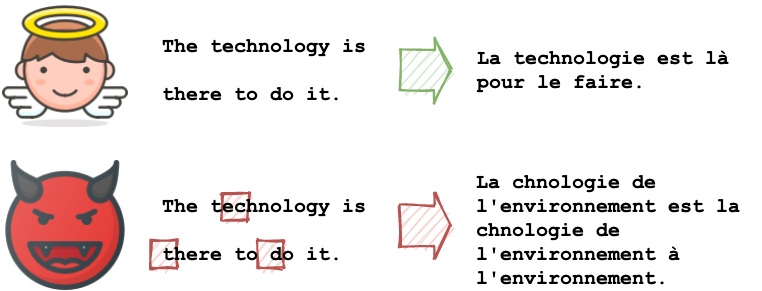
\includegraphics[scale=0.599]{figures/invisible.png}
  \caption{Hyökkäys näkymättömillä merkeillä \citep{boucher2021bad}}
\end{figure}

\section{Homoglyfit}
Homoglyfihyökkäykset NLP-luokittimia vastaan pohjautuvat siihen, että pahantahtoisten\\ merkkien viralliset esitysmuodot näyttäytyvät hyväntahtoisilta merkkien virallisilta esityksiltä. Jois\-sain kielissä tekstin merkitys muuttuu täysin yhden merkin vaihtuessa. Esimerkkinä homoglyfistä on \texttt{A $\rightarrow$ A}, missä viimeinen kirjain on todellisuudessa kyrillinen kirjain A. Kuvassa 3.2 homoglyfihyökkäys on muuntanut englanninkielisen tekstin\\ \texttt{I just can't belive where she was} ranskankieliseen käännökseen\\ \texttt{I guess I can't underestimate the location of the scribe and}.
\begin{figure}[hbt]
  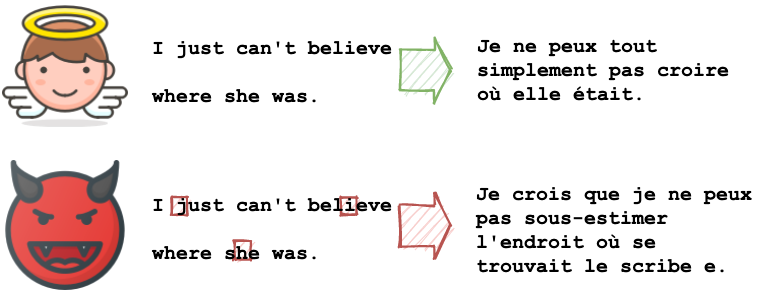
\includegraphics[scale=0.599]{figures/homoglyph.png}
  \caption{Homoglyfihyökkäys \citep{boucher2021bad}}
\end{figure}
\\Näkymättömien merkkien lailla homoglyfihyökkäyksen toteutus riippuu ympäristön fontista. \citep{boucher2021bad}

\section{Uudelleenjärjestelyt}
Uudelleenjärjestelyhyökkäys pohjautuu näennäisen tekstin uudelleenjärjestämiseen pahantahtoisesti. Pankkitilinumeron \texttt{1234567} pystyy esimerkiksi vaihtamaan kaksisuuntaisella-algoritmilla tilinumeroksi \texttt{7654321} pankin palvelinpuolella maksajan huomaamatta mitään. Unicode-merkintä tälle suunnanvaihdolle on \texttt{U+200F}. Uudelleenjärjestelyjä käytetään myös NLP-luokittimen sekoittamiseen, jolloin tulokset NLP-luokittimesta ovat käyttökelvottomia. Kuvassa 3.3 uudelleenjärjestelyhyökkäys merkeissä \texttt{la} aiheuttaa ranskankielisen käännöksen järjettömyyden. Tämänlaista hyökkäystä voisi käyttää digitaalista sanakirjaa tai kääntäjää vastaan. \citep{boucher2021bad}
\begin{figure}[t]
  
\includegraphics[scale=0.599]{figures/reordering.png}
  \caption{Homoglyfihyökkäys \citep{boucher2021bad}}
\end{figure}
\texttt{U+200F} ladotaan näkymättömänä näkymättömien merkkien tapaan.

\section{Poistatukset}

Viimeisenä käydään läpi poistatushyökkäykset. Poistatushyökkäyksen tarkoituksena on poistaa käyttäjälle näkyvästä tekstistä ladontavaiheessa haluttu määrä tekstiä pois. Uhri esimerkiksi voisi olla myymässä pois asuntoaan, jolloin tämä kopioi ja liittää sähköiseen sopimukseen hyökkääjän ehdottaman summan. Latomisvaiheessa käyttäjä kuitenkin unohtaa tarkistaa sopimuksen, jolloin poistatusmerkit saattavat poistaa myyntihinnasta esimerkiksi muutaman nollan.

Poistatushyökkäyksiä on vaikeampi toteuttaa aikaisempiin metodeihin verrattuna. Tämä johtuu useimpien käyttöjärjestelmien estosta kopioida poistatusta sisältävää tekstiä leikepöydälle suoraviivaisilla tavoilla, joilla uhri sen tekisi. Onnistuakseen poistatushyökkäyksessä, hyökkääjän tarvitsee yleisesti injektoida NLP-luokittimeen poistatus itse. Esimerkkejä poistatusmerkeistä ovat askelpalautin (BS, eng. backspace), delete (DEL) sekä vaununpalautus (CR, eng. carriage return). \citep{boucher2021bad}
Kuva 3.4 havainnollistaa poistatushyökkäystä käytännössä. Esimerkissä poistatusmerkkejä on pistetty sanojen väliin, muuttaen näin ladottujen lauseiden merkityksen.
\begin{figure}[t]
  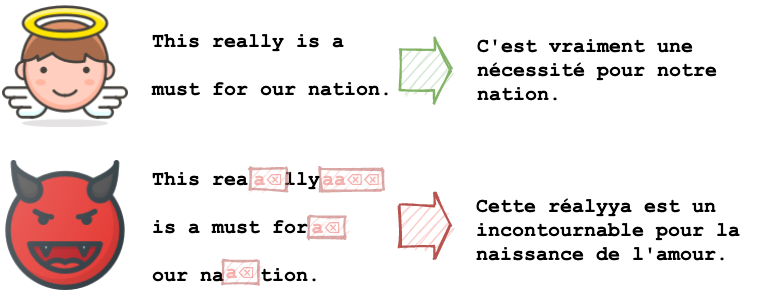
\includegraphics[scale=0.599]{figures/backspace.png}
  \caption{Poistatushyökkäys \citep{boucher2021bad}}
\end{figure}